\documentclass[master=cws,masteroption=mmc, bind=18mm]{kulemt}
%\documentclass[master=cws,masteroption=mmc,oneside]{kulemt}
\setup{title={Het gebruik van de normalen bij het bouwen van BSP acceleratiestructuren},
  author={Jesse Hoobergs},
  promotor={Prof.\,dr.\,ir.\ Ph. Dutré},
  assessor={Dr. B. Verreet\and Prof. dr. R. Vandebril},
  assistant={Ir. P. Bartels}}
% De volgende \setup mag verwijderd worden als geen fiche gewenst is.
\setup{filingcard,
  translatedtitle={Using the normals to build BSP acceleration structures.},
  udc=681.3,
  shortabstract={In deze masterproef introduceren we een nieuw soort algemene Binary Space Partitioning ($\symBSP$) boom: de $\symBSPsweep$ boom.  De $\symBSPsweep$ boom laat toe om in elke knoop een aantal richtingen te bepalen afhankelijk van de driehoeken in die knoop  en het beste vlak van alle vlakken met als normaal één van die richtingen, wordt gebruikt om de knoop te splitsen.  Drie soorten $\symBSPsweep$ boom zijn ontworpen: één soort die in elke knoop random richtingen genereert ($\symBSPrandom$) en twee soorten die richtingen genereren afhankelijk van de normalen van de driehoeken in de knoop ($\symBSParbitrary$ en $\symBSPcluster$).  De $\symBSParbitrary$ boom kiest de normalen van enkele willekeurige driehoeken in de knoop als richtingen en de $\symBSPcluster$ boom bepaalt een clustering van de normalen van de driehoeken in de knoop en gebruikt de centra van deze clusters als richtingen.  Er is ook een optimalisatie van de $\symBSPsweep$ boom uitgewerkt: de $\symBSPsweepfastkd$ boom die asgealigneerde splitsingsvlakken bevoordeeld omdat ze computationele voordelen hebben.\\
  De drie $\symBSPsweepfastkd$ soorten zijn duidelijk beter dan de bestaande $\symBSP$ bomen. Van de drie soorten $\symBSPsweepfastkd$ bomen zijn de twee soorten die gebruik maken van de normalen, beduidend beter dan de soort die random richtingen bepaalt. Ze verminderen bij alle testscenes het aantal straal-driehoekintersecties met meer dan 40\% en de rendertijd met meer dan 20\% ten opzichte van de $\symKd$ boom. De bouwtijd is twee ordegroottes groter dan die van de $\symKd$ boom, maar wel kleiner dan die van elke andere $\symBSP$ boom.}}
% Verwijder de "%" op de volgende lijn als je de kaft wil afdrukken
%\setup{coverpageonly}
% Verwijder de "%" op de volgende lijn als je enkel de eerste pagina's wil
% afdrukken en de rest bv. via Word aanmaken.
%\setup{frontpagesonly}

% Kies de fonts voor de gewone tekst, bv. Latin Modern
\setup{font=lm}
\setup{inputenc=utf8}

\usepackage{tikz-qtree}
\definecolor{nodeblue1}{HTML}{44FFFF}
\definecolor{nodeblue2}{HTML}{2D00AF}
\definecolor{nodered1}{HTML}{DF2D00}
\definecolor{nodered2}{HTML}{FF4488}
\definecolor{nodered3}{HTML}{EF5D00}
\definecolor{nodered4}{HTML}{FF8888}
\definecolor{nodeyellow1}{HTML}{FFFF00}
\usepackage{subcaption}
\captionsetup{compatibility=false}
\usepackage{csvsimple}
\usepackage{pgfplots}
\usepackage{listings}
\usepackage{algorithm}
\usepackage{algorithmicx}
\usepackage{algpseudocode}
\usepackage{xspace}
\algnewcommand{\And}{\textbf{and}\xspace}
\algnewcommand{\Or}{\textbf{or}\xspace}

\usepackage{colortbl}
\usepackage{pgfplotstable}
\usepackage{siunitx}

\pgfplotstableset{
    /color cells/min/.initial=0,
    /color cells/max/.initial=1000,
    /color cells/textcolor/.initial=,
    %
    % Usage: 'color cells={min=<value which is mapped to lowest color>, 
    %   max = <value which is mapped to largest>}
    color cells/.code={%
        \pgfqkeys{/color cells}{#1}%
        \pgfkeysalso{%
            postproc cell content/.code={%
                %
                \begingroup
                %
                % acquire the value before any number printer changed
                % it:
                \pgfkeysgetvalue{/pgfplots/table/@preprocessed cell content}\value
                \ifx\value\empty
                    \endgroup
                \else
                \pgfmathfloatparsenumber{\value}%
                \pgfmathfloattofixed{\pgfmathresult}%
                \let\value=\pgfmathresult
                %
                % map that value:
                \pgfplotscolormapaccess
                    [\pgfkeysvalueof{/color cells/min}:\pgfkeysvalueof{/color cells/max}]
                    {\value}
                    {\pgfkeysvalueof{/pgfplots/colormap name}}%
                % now, \pgfmathresult contains {<R>,<G>,<B>}
                % 
                % acquire the value AFTER any preprocessor or
                % typesetter (like number printer) worked on it:
                \pgfkeysgetvalue{/pgfplots/table/@cell content}\typesetvalue
                \pgfkeysgetvalue{/color cells/textcolor}\textcolorvalue
                %
                % tex-expansion control
                % see https://tex.stackexchange.com/questions/12668/where-do-i-start-latex-programming/27589#27589
                \toks0=\expandafter{\typesetvalue}%
                \xdef\temp{%
                    \noexpand\pgfkeysalso{%
                        @cell content={%
                            \noexpand\cellcolor[rgb]{\pgfmathresult}%
                            \noexpand\definecolor{mapped color}{rgb}{\pgfmathresult}%
                            \ifx\textcolorvalue\empty
                            \else
                                \noexpand\color{\textcolorvalue}%
                            \fi
                            \the\toks0 %
                        }%
                    }%
                }%
                \endgroup
                \temp
                \fi
            }%
        }%
    }
}

\newenvironment{dutchalgorithm}[1][]
  {\begin{algorithm}[#1]
     \selectlanguage{dutch}%
     \floatname{algorithm}{Algoritme}%
     \renewcommand{\algorithmicif}{\textbf{if}}%
     \renewcommand{\algorithmicthen}{\textbf{then}}%
     \renewcommand{\algorithmicend}{\textbf{end}}%
     % Set other language requirements
  }
  {\end{algorithm}}
  \renewcommand{\listalgorithmname}{Lijst van algoritmen}

\newcommand\symO{\mathcal{O}}
\newcommand\symSA{\mathcal{SA}}
\newcommand\symCost{\mathcal{K}}
\newcommand\symLeft{l}
\newcommand\symRight{r}
\newcommand\symNbPrimitives{n}
\newcommand\symIntersection{i}
\newcommand\symTraversal{d}
\newcommand\symNodeExample{p}
\newcommand\symBSP{BSP}
\newcommand\symKd{Kd}
\newcommand\symCostTraversalBSP{\symCost_{\symTraversal,\symBSP}}
\newcommand\symCostTraversalKd{\symCost_{\symTraversal,\symKd}}

\newcommand\authorKammaje{Kammaje and Mora}
\newcommand\authorIze{Ize et al}

% Hier kun je dan nog andere pakketten laden of eigen definities voorzien

% Tenslotte wordt hyperref gebruikt voor pdf bestanden.
% Dit mag verwijderd worden voor de af te drukken versie.
\usepackage[pdfusetitle,hidelinks,plainpages=false]{hyperref}

%%%%%%%
% Om wat tekst te genereren wordt hier het lipsum pakket gebruikt.
% Bij een echte masterproef heb je dit natuurlijk nooit nodig!
\IfFileExists{lipsum.sty}%
 {\usepackage{lipsum}\setlipsumdefault{11-13}}%
 {\newcommand{\lipsum}[1][11-13]{\par Hier komt wat tekst: lipsum ##1.\par}}
%%%%%%%

%\includeonly{hfdst-n}
\begin{document}

\begin{preface}
  Het maken van een masterproef is een uitdaging die je niet alleen aangaat. Ik zou daarom dit voorwoord in de eerste plaats willen gebruiken om mijn promotor Philip Dutré te bedanken om dit onderwerp ter beschikking te stellen, voor de vrijheid waarmee ik dit onderwerp mocht aanpakken en voor de nuttige feedback en discussies tijdens de tussentijdse presentaties.
  Verder wil ik Matthias Moulin bedanken voor de uitstekende begeleiding in het eerste semester en Pieterjan Bartels om deze taak in het tweede semester met glans over te nemen. Ze hebben me met hun feedback geholpen bij het vormgeven van de ontwikkelde methoden en deze thesistekst. Hiernaast wil ik nog graag de voltallige jury bedanken voor het lezen van deze thesis.\\

  Tot slot wil ik graag mijn familie en vrienden bedanken voor hun steun tijdens dit volledige academiejaar. In het bijzonder wil ik Jens Claes en Jorik Jooken bedanken om deze thesistekst na te lezen.
\end{preface}

\tableofcontents*

\begin{abstract}
\textit{Ray tracing} is een computergrafiek techniek waarbij stralen door een virtuele 3D scene gestuurd worden om een realistische 2D afbeelding te genereren.
Om het aantal straal-driehoekintersecties te verminderen, wordt gebruik gemaakt van acceleratiestructuren.
Acceleratiestructuren zorgen dat stralen enkel geïntersecteerd worden met driehoeken die mogelijks snijden.
Eén van de meestgebruikte acceleratiestructuren zijn  \textit{Binary Space Partitioning} ($\symBSP$) bomen.
Bij de $\symBSP$ boom wordt het omhullend volume van de scene recursief opgesplitst in kindvolumes via een splitsingsvlak.
In de praktijk wordt altijd de $\symKd$ boom gebruikt, een specifiek soort $\symBSP$ boom, die enkel splitst via asgealigneerde splitsingsvlakken.\\

In deze masterproef introduceren we een nieuw soort algemene $\symBSP$ boom: de $\symBSPsweep$ boom.
De $\symBSPsweep$ boom laat toe om in elke knoop een aantal richtingen te bepalen afhankelijk van de driehoeken in die knoop.
Het beste vlak van alle vlakken met als normaal één van die richtingen, wordt gebruikt om de knoop te splitsen.
Drie soorten $\symBSPsweep$ boom zijn ontworpen: één soort die in elke knoop random richtingen genereert ($\symBSPrandom$) en twee soorten die richtingen genereren afhankelijk van de normalen van de driehoeken in de knoop ($\symBSParbitrary$ en $\symBSPcluster$).
De $\symBSParbitrary$ boom kiest de normalen van enkele willekeurige driehoeken in de knoop als richtingen en de $\symBSPcluster$  boom bepaalt een clustering van de normalen van de driehoeken in de knoop en gebruikt de centra van deze clusters als richtingen.
Er is ook een optimalisatie van de $\symBSPsweep$ boom uitgewerkt: de $\symBSPsweepfastkd$ boom die asgealigneerde splitsingsvlakken bevoordeeld omdat ze computationele voordelen hebben.\\

De drie $\symBSPsweepfastkd$ soorten zijn duidelijk beter dan de bestaande $\symBSP$ bomen. 
Van de drie soorten $\symBSPsweepfastkd$ bomen zijn de twee soorten die gebruik maken van de normalen, beduidend beter dan de soort die random richtingen bepaalt.
Ze verminderen bij alle testscenes het aantal straal-driehoekintersecties met meer dan 40\% en de rendertijd met meer dan 20\% ten opzichte van de $\symKd$ boom. De bouwtijd is twee ordegroottes groter dan die van de $\symKd$ boom, maar wel kleiner dan die van elke andere algemene $\symBSP$ boom.
\end{abstract}

% Een lijst van figuren en tabellen is optioneel
\listoffigures
\listoftables
\listofalgorithms
\addcontentsline{toc}{chapter}{Lijst van algoritmen}
% Bij een beperkt aantal figuren en tabellen gebruik je liever het volgende:
%\listoffiguresandtables
% De lijst van symbolen is eveneens optioneel.
% Deze lijst moet wel manueel aangemaakt worden, bv. als volgt:
\chapter{Lijst van afkortingen en symbolen}
\section*{Afkortingen}
\begin{flushleft}
  \renewcommand{\arraystretch}{1.1}
  \begin{tabularx}{\textwidth}{@{}p{20mm}X@{}}
    $\symBSP$ & Binary Space Partitioning \\
    $\symBVH$ & Bounding Volume Hierarchy \\
    $\symKDOP$ & Discrete Oriented Polytope met $k$ richtingen \\
    $\symRBSP$ & Restricted Binary Space Partitioning \\
    $\symSA$   & Surface Area \\
    $\symSAH$  & Surface Area Heuristiek \\
  \end{tabularx}
\end{flushleft}
\pagebreak
%\chapter{Lijst van symbolen}
\section*{Symbolen}
\begin{flushleft}
  \renewcommand{\arraystretch}{1.1}
  \begin{tabularx}{\textwidth}{@{}p{25mm}X@{}}
    $\alpha$ & Een parameter om $\symCostTraversalBSP$ lineair te laten variëren met het aantal driehoeken. \\
    $\beta$ & Het procentueel aantal doorkruisingen door een inwendige knoop dat door slechts één van de twee kindknopen gaat. \\
    $\symBSParbitrary$ & $\symBSP$ boom die per knoop willekeurige normalen als splitsingsrichtingen gebruikt. \\
    $\symBSParbitrarykd$ & $\symBSParbitrary$ boom waarbij de drie richtingen volgens de hoofdassen altijd deel uitmaken van de splitsingsrichtingen. \\
    $\symBSParbitraryfastkd$ & $\symBSParbitrarykd$ boom waarbij $\symKd$ knopen efficiënter doorkruist worden dan $\symBSP$ knopen. \\
    $\symBSPcluster$ & $\symBSP$ boom die per knoop een clustering van de normalen berekent en de centra van deze clusters als splitsingsrichtingen gebruikt. \\
    $\symBSPclusterkd$ & $\symBSPcluster$ boom waarbij de drie richtingen volgens de hoofdassen altijd deel uitmaken van de splitsingsrichtingen. \\
    $\symBSPclusterfastkd$ & $\symBSPclusterkd$ boom waarbij $\symKd$ knopen efficiënter doorkruist worden dan $\symBSP$ knopen. \\
    $\symBSPrandom$ & $\symBSP$ boom die per knoop random richtingen als splitsingsrichtingen gebruikt. \\
    $\symBSPrandomkd$ & $\symBSPrandom$ boom waarbij de drie richtingen volgens de hoofdassen altijd deel uitmaken van de random splitsingsrichtingen. \\
    $\symBSPrandomfastkd$ & $\symBSPrandomkd$ boom waarbij $\symKd$ knopen efficiënter doorkruist worden dan $\symBSP$ knopen. \\
    $k$ & Het aantal splitsingsrichtingen dat in elke knoop bekeken wordt. \\
    $\symCostTraversal$ & De kost om een inwendige knoop te doorkruisen. \\
    $\symCostTraversalBSP$ & De kost om een inwendige BSP knoop te doorkruisen. \\
    $\symCostTraversalKd$ & De kost om een inwendige Kd knoop te doorkruisen. \\
    $\symCost_{\symIntersection}$ & De kost te intersecteren met een primitief. \\
    $\symNbPrimitives$ & Het aantal primitieven\\
    $\symTime_{\symTraversal}$ & De tijd nodig om één inwendige knoop te doorkruisen. \\
    $\symTime_{\symTraversal, \symTotal}$ & De totale tijd gespendeerd aan het doorkruisen van een boom. \\
    $\symTime_{\symIntersection}$ & De tijd nodig om te intersecteren met één primitief. \\
    $\symTime_{\symIntersection, \symTotal}$ & De totale tijd gespendeerd aan het intersecteren met primitieven. \\
    $\symTime_{\symRender}$ & De rendertijd\\
    $\symRBSPKd$ & $\symRBSP$ boom waarbij $\symKd$ knopen efficiënter doorkruist worden dan $\symBSP$ knopen. \\
  
  \end{tabularx}
\end{flushleft}

% Nu begint de eigenlijke tekst
\mainmatter

\chapter{Inleiding}
\label{hoofdstuk:inleiding}
In dit hoofdstuk wordt het werk ingeleid. Het doel wordt gedefinieerd en er
wordt uitgelegd wat de te volgen weg is (beter bekend als de rode draad).

Als je niet goed weet wat een masterproef is, kan je altijd
Wikipedia eens nakijken.

\section{Ray tracing}
    \paragraph{Stralen volgen}
    Door elke pixel één (of meerdere stralen), kleur intersectiepunt is kleur pixel -> path tracing.
    \paragraph{Acceleratiestructuren}
    Doel: aantal straal-driehoek intersecties verminderen.
\section{Doelstelling}
Betere Acceleratiestructuur bouwen door een algemene BSP te maken die gebruik maakt van de geometrische normalen bij het splitsen. 
Aantal intersecties nog doen dalen, traversals stijgen, rendertijd dalen.
\section{Methodologie}
\section{Contributie}
\section{Overzicht}

%%% Local Variables: 
%%% mode: latex
%%% TeX-master: "masterproef"
%%% End: 

\chapter{Voorgaand werk}
\label{hoofdstuk:voorgaand-werk}
Raytracing vereist acceleratiestructuren om efficiënt driehoeken in de scene te kunnen zoeken.
Dit hoofdstuk start met een algemene uitleg over acceleratiestructuren en wijdt dan uit over één specifieke acceleratiestructuur: de \textit{Binary Space Partitioning} ($\symBSP$) boom.
De varianten van de $\symBSP$ boom worden één voor één besproken.
% TODO

\section{Basisconcept}
    
    % TODO: raytracing
    \paragraph{Ray tracing}
    \textit{Ray tracing} is een computergrafiek techniek voor fysisch gebaseerd renderen. Het vormt een beschrijving van een 3D scene om tot een fotorealistische 2D afbeelding. Een camera wordt op een bepaalde positie in de scene geplaatst en een afbeeldingsvlak, opgedeeld in pixels, wordt ervoor geplaatst. Door elke pixel worden één (of meerdere stralen) gestuurd. Deze stralen worden zichtstralen genoemd en de kleur van hun dichtste intersectiepunt met de scene, bepaalt de kleur van de pixel.\\

    \begin{figure}
        \centering
        \includegraphics[width=0.5\linewidth]{img/ray-tracing}
        \caption{Een visuele voorstelling van \textit{ray tracing}. Door elke pixel worden één of meerdere zichtstralen gestuurd. Schaduwstralen worden gebruikt om de belichting in de scene realistisch te maken. Deze afbeelding is een aangepaste versie van een afbeelding op \url{https://en.wikipedia.org/wiki/Ray_tracing_(graphics)}}
        \label{fig:raytracing}    
    \end{figure}

    Om realistische afbeeldingen te maken, wordt belichting in rekening gebracht. De eenvoudigste vorm van belichting is directe belichting, een punt is donker als er niet rechtstreeks licht van een lichtbron op valt. Om dit te ondersteunen in \textit{ray tracing} wordt gebruikt gemaakt van schaduwstralen, stralen van het punt naar de lichtbron.  Deze schaduwstralen worden geïntersecteerd met de scene, als een intersectiepunt tussen het punt en de lichtbron gevonden wordt, is de lichtbron niet zichtbaar.  Bij elke intersectie wordt aan de hand van schaduwstralen gekeken of het punt belicht wordt of niet, als het niet belicht wordt, is de kleur zwart. Voor indirecte belichting kan een andere techniek, \textit{path tracing}, gebruikt worden. \textit{Path tracing} reflecteert stralen in het intersectiepunt afhankelijk van het materiaal en als deze straal na een aantal botsingen een lichtbron raakt, krijgt het intersectiepunt een belichting van die lichtbron.    
    
  %  , kleur intersectiepunt is kleur pixel -> path tracing.
  %  voor realistische beeldgeneratie + referentie,


    \paragraph{Acceleratiestructuren}
    Het doel van acceleratiestructuren is om het aantal straal-driehoek intersecties te verminderen.
    De simpelste acceleratiestructuur bestaat uit het omhullende volume van de scene.
    Testen op intersectie met de driehoeken in de scene gebeurt dan enkel als dit omhullende volume intersecteert met de straal.
    Deze acceleratiestructuur kan worden uitgebreid tot een boomstructuur door dit volume recursief op te delen in kindvolumes.
    Binaire bomen delen elk omhullend volume op in twee nieuwe volumes, andere acceleratiestructuren zoals bijvoorbeeld octrees, delen het volume op in meer dan twee volumes.
    \\

    Het volume kan worden opgedeeld op twee manieren: volgens objecten of volgens ruimte.
    Bij opdeling volgens objecten worden de objecten binnen het volume opgedeeld in meerdere disjuncte groepen en de kindvolumes zijn de omhullende volumes van deze groepen.
    Na deze opdeling zit elk object in exact één van deze nieuwe volumes, maar de volumes kunnen overlappen.
    Een voorbeeld van een acceleratiestructuur waarbij de opdeling volgens objecten gebeurt is de \textit{Bounding Volume Hierarchy} ($\symBVH$).
    Opdeling volgens ruimte betekent dat de ruimte in het volume wordt opgedeeld in meerdere delen.
    Na deze opdeling overlappen deze nieuwe volumes niet, maar een object ligt nu in minstens één (en mogelijks in meerdere) kindvolume(s).
    De $\symBSP$ boom deelt de ruimte van het volume steeds op in twee kindvolumes.
    % TODO: combinatie van Kd en BVH ? SBVH
    % TODO: check if all abbrev are listed and defined at first usage

\section{$\symBSP$ bomen}
    De $\symBSP$ boom deelt de ruimte van het omhullende volume recursief op door te splitsen volgens een willekeurig georiënteerd vlak totdat een bepaalde stopconditie bereikt is.
    Het feit dat de $\symBSP$ boom volgens willekeurig georiënteerde vlakken splitst, is zowel een voor- als nadeel.
    Het zorgt ervoor dat de $\symBSP$ boom zich heel goed kan aanpassen aan de scene en alle niet-intersecterende driehoeken in principe kan scheiden (zie figuur \ref{fig:splitsing-bsp}).
    Maar het zorgt er ook voor dat het heel moeilijk is om deze goede splitsingsvlakken te vinden.
    In de praktijk wordt vaak een specifieke soort $\symBSP$ boom gebruikt: de $\symKd$ boom.
    \begin{figure}
        \centering
        \includegraphics[width=\linewidth]{img/splitsing-BSP}
        \caption{Een 2D voorbeeld dat toont dat alle (niet-intersecterende) driehoeken gesplitst kunnen worden door een $\symBSP$ boom.}
        \label{fig:splitsing-bsp}    
    \end{figure}    
    \paragraph{Het bouwen van de boom}
    Het splitsingsvlak dat een knoop opdeelt in twee delen, kan een grote impact hebben op het aantal doorkruisstappen en het aantal driehoekintersecties.
    Het bouwalgoritme moet voor elke knoop het beste splitsingvlak bepalen en als splitsen volgens dat vlak voordelig is, de knoop opsplitsen in twee kindknopen.
    Heuristieken voorspellen hoe goed een splitsing volgens een bepaald splitsingsvlak is.   
    Het algoritme stopt met het splitsen van de knoop als een stopconditie bereikt wordt.
    Deze stopconditie kan een maximale diepte zijn, of het feit dat er geen nuttig splitsingsvlak gevonden wordt of dat het aantal driehoeken in de knoop lager is dan een vastgelegde limiet, bijvoorbeeld als er maar één driehoek in de knoop zit.

    %Spatiaal, opsplitsen volgens willekeurige vlakken
    %Niet feasible geacht
   
\section{$\symKd$ Bomen}   
    De $\symKd$ boom is een $\symBSP$ boom waarbij alle splitsingsvlakken asgealigneerd zijn.
    Hiermee wordt bedoeld dat de splitsingsrichting (de normaal op het splitsingsvlak) evenwijdig is aan één van de drie hoofdassen.
    Dit zorgt ervoor dat elke knoop van de boom een asgealigneerde balk voorstelt.
    Het doorkruisen van een knoop uit een $\symKd$ boom is daardoor goedkoper dan het doorkruisen van een knoop uit een algemene $\symBSP$ boom.
    De reden hiervoor is dat het goedkoper is om het intersectiepunt van een straal en een asgealigneerd vlak te vinden (verschil en vermenigvuldiging) dan het intersectiepunt van een straal en een willekeurig vlak (twee scalaire producten en deling).
    Door de beperking op mogelijke splitsingsvlakken kunnen $\symKd$ bomen zich minder goed aanpassen aan de scene.
    Ze kunnen bijvoorbeeld niet alle niet-intersecterende driehoeken scheiden. 
    Figuur \ref{fig:splitsing-kd} toont een situatie waarin de $\symKd$ boom niet alle driehoeken kan scheiden.
    \\ % TODO: 2D voorbeeld van splitsbaar en wat niet

    \begin{figure}
        \centering
        \includegraphics[width=\linewidth]{img/splitsing-Kd}
        \caption{Een 2D voorbeeld dat toont dat niet alle (niet-intersecterende) driehoeken gesplitst kunnen worden door de asgealigneerde vlakken van de $\symKd$ boom. De twee driehoeken linksonder (en rechtsboven) kunnen niet gesplitst worden omdat zowel hun projecties op de x-as, als hun projecties op de y-as overlappen.}
        \label{fig:splitsing-kd}    
    \end{figure}

    Ondanks dit nadeel, worden in de praktijk $\symKd$ bomen verkozen boven algemene $\symBSP$ bomen.
    \authorIze{} \cite{ize} geven drie (volgens hun foute) ruimverspreide aannames over algemene $\symBSP$ bomen die ervoor zorgen dat $\symKd$ bomen hoger ingeschat worden.
    Ten eerste wordt er aangenomen dat algemene $\symBSP$ bomen nooit sneller kunnen zijn dan $\symKd$ bomen omdat het doorkruisen van een $\symBSP$ boom beduidend duurder is.
    De beperkte precisie van vlottende komma getallen wordt gezien als het tweede probleem omdat het $\symBSP$ bomen numeriek onstabiel zou maken.
    De derde aanname is dat door de grotere flexibileit (= grotere verzameling van mogelijke splitsingsvlakken) het veel moeilijker is om een $\symBSP$ boom te bouwen dan om een $\symKd$ boom te bouwen.
    \\

    Voor een Kd-boom is de Surface Area Heuristiek ($\symSAH$) de beste gekende methode om bomen met minimale verwachtte kost te bouwen.
    De $\symSAH$ is oorspronkelijk ontwikkelt door \authorGoldsmithSalmon{} \cite{goldsmith1987automatic} voor de $\symBVH$ en later aangepast door \authorMacDonaldBooth{} \cite{macdonald1990heuristics} voor de $\symKd$ boom. 
    De $\symSAH$ schat de kost van een splitsingsvlak door te veronderstellen dat beide kindknopen, bladknopen worden en dat de kost om een bladknoop te intersecteren afhankelijk is van het aantal driehoeken en de oppervlakte van het omhullende volume.
    De verwachte kost $\symCost$ om een knoop $\symNodeExample$ te splitsen in kindknopen ${\symLeft}$ en ${\symRight}$ is dan: $\symCost_\symNodeExample = \frac{\symSA(\symLeft)}{\symSA(\symNodeExample)}*\symNbPrimitives_\symLeft*\symCost_\symIntersection + \frac{\symSA(\symRight)}{\symSA(\symNodeExample)}*\symNbPrimitives_\symRight*\symCost_\symIntersection + \symCost_\symTraversal$ met kost $\symCost$, oppervlakte $\symSA()$ en aantal driehoeken $\symNbPrimitives$.
    De subscripts ${\symIntersection}$ en ${\symTraversal}$ staan voor respectievelijk intersectie en doorkruising.
    De kost van het beste splitsingsvlak (laagste kost) wordt dan vergeleken met de kost voor de knoop als die niet gesplitst zou worden: $\symNbPrimitives*\symCost_\symIntersection$.
    Als splitsen voordelig is, wordt de knoop opgesplitst volgens dit splitsingsvlak, anders wordt de knoop een bladknoop.
    \\

    Alle mogelijke asgealigneerde splitsingsvlakken testen is ondoenbaar. 
    \authorHavran{} \cite{havran2000heuristic} toonde aan dat de kost van de $\symSAH$ langs een richting ofwel lineair stijgt ofwel linear daalt tussen eindpunten (de minimale en maximale waarde) van de driehoeken langs die richting.
    Dit impliceert dat het beste splitsingsvlak door een eindpunt van een driehoek gaat.
    Het is dus voldoende om enkel de splitsingsvlakken te bekijken die door de eindpunten van de driehoeken gaan.
    Hieruit volgt dat er voor elke richting in een knoop met $n$ driehoeken, $2n$ splitsingsvlakken bekeken moeten worden.
    Bij een $\symKd$ boom is het dus voldoende om $6n$ splitsingsvlakken te bekijken.
    Om de $\symSAH$ kost te berekenen voor een splitsingsvlak moet het aantal driehoeken dat (deels) aan de ene kant van het splitsingsvlak ligt ($\symNbPrimitives_\symLeft$) en het aantal driehoeken dat (deels) aan de andere kant ligt ($\symNbPrimitives_\symRight$) gekend zijn.
    Om deze aantallen efficiënt te kunnen berekenen, worden de eindpunten van de driehoeken in de knoop gesorteerd volgens hun projectie op de splitsingsrichting.
    Een veegbeweging (\textit{sweep}) over deze gesorteerde lijst kan dan in lineaire tijd de $SAH$ kost van alle splitsingsvlakken langs de splitsingsrichting berekenen.

    % nulbonus ?
\section{$\symRBSP$ bomen}
    De Restricted Binary Space Partitioning ($\symRBSP$) boom is een uitbreiding van de $\symKd$ boom die toelaat om knopen op te splitsen volgens splitsingsrichtingen uit een vaste verzameling van k richtingen.
    Het omhullend volume van een $\symRBSP$ knoop is hierdoor geen balk maar een Discreet Geöriënteerde Polytoop met k richtingen: een \symKDOP.
    Zowel \authorKlosowki{} \cite{klosowski1998efficient} als \authorZachmann{} \cite{zachmann1998rapid} hebben hiërarchiën van \symKDOP s gebruikt binnen het domein van botsherkenning (\textit{collision detection}).
    De $\symRBSP$ boom is voor het eerst gebruikt in ray tracing door \authorKammaje{} \cite{Kammaje} en verder onderzocht door \authorBudge{} \cite{Budge}.
    Aangezien de splitsingsrichtingen niet asgealigneerd moeten zijn, lijkt de $\symRBSP$ boom meer op de algemene $\symBSP$ boom dan de $\symKd$ boom. Net als de $\symKd$ boom kan de $\symRBSP$ boom niet alle niet-intersecterende driehoeken scheiden. 
    Figuur \ref{fig:splitsing-rbsp} toont een situatie waarin de $\symRBSP$ boom niet alle driehoeken kan scheiden.
    \\

    \begin{figure}
        \centering
        \includegraphics[width=\linewidth]{img/splitsing-RBSP}
        \caption{Een 2D voorbeeld dat toont dat niet alle (niet-intersecterende) driehoeken gesplitst kunnen worden door de vlakken van de $\symRBSP$ boom. De $\symRBSP$ boom kan de driehoeken wel beter splitsen dan de $\symKd$ boom in figuur \ref{fig:splitsing-kd}. De twee driehoeken rechtsboven kunnen niet gesplitst worden omdat de discrete verzameling van k richtingen, geen richting bevat waarlangs deze driehoeken gesplitst kunnen worden.}
        \label{fig:splitsing-rbsp}    
    \end{figure}

    Een belangrijke ontwerpbeslissing bij $\symRBSP$ bomen is het kiezen van de verzameling splitsingsrichtingen. 
    Volgens \authorBudge{} \cite{Budge} werkt in principe elke verzameling met minstens drie niet-evenwijdige richtingen, maar is het gewenst om richtingen te kiezen die samen de eenheidsbol goed bedekken.
    \authorKammaje{} \cite{Kammaje} genereren punten langs een spiraal op gelijk verdeelde breedtegraden volgens de gouden ratio.
    \authorBudge{} \cite{Budge} gebruiken de verzamelingen die ze de standaard richtingen van \authorKlosowki{} \cite{klosowski1998efficient} noemen.
    Deze richtingen gebruiken enkel waarden uit de verzameling $\{-1, 0, 1\}$ als x, y en z coördinaat. %TODO meer uitwijden ?
    \\

    \authorKammaje{} \cite{Kammaje} toonden aan dat de SAH ook gebruikt kan worden voor $\symRBSP$ bomen. Net zoals bij de $\symKd$ boom moeten voor elke splitsingsrichting de eindpunten van de driehoeken gesorteerd worden en $2n$ splitsingsvlakken bekeken worden. In totaal bekijkt de $\symRBSP$ boom dus $2kn$ splitsingsvlakken. Het bouwen van de $\symRBSP$ boom is computationeel duurder dan het bouwen van de $\symKd$ boom door het grotere aantal richtingen en het feit dat het berekenen van de oppervlakte van een \symKDOP{} computationeel duurder is dan het berekenen van de oppervlakte van een balk. \authorBudge{} \cite{Budge} vonden een oplossing voor dit tweede probleem door een methode te ontwikkelen waarmee de oppervlaktes van de kind \symKDOP s incrementeel berekend kunnen worden tijdens het sweepen.\\

    De huidige $\symRBSP$ implementaties zijn superieur ten opzichte van de $\symKd$ boom in termen van het aantal driehoekintersecties en het aantal doorkruisingen, maar moet onderdoen in termen van rendertijd.
    \authorIze{} \cite{ize} menen dat de $\symRBSP$ boom de slechtste eigenschappen van zowel de $\symKd$ boom als de algemene $\symBSP$ boom overneemt. 
    Net als de $\symKd$ boom kan het geen rekening houden met de lokale geometrie en zich dus niet aanpassen aan complexe geometrie.
    Net als bij de algemene $\symBSP$ boom moet de intersectie met een willekeurig georiënteerd vlak berekend worden om knopen te doorkruisen. \authorBudge{} \cite{Budge} tonen aan dat deze tweede eigenschap minder erg is bij de $\symRBSP$ boom dan bij de algemene $\symBSP$ boom omdat het mogelijk is om alle scalaire producten op voorhand (en dus maar één keer) te berekenen.

\section{Algemene $\symBSP$ Bomen in de praktijk}
    \authorIze{} \cite{ize} ontwikkelden de eerste algemene $\symBSP$ boom voor raytracing. In tegenstelling tot de $\symKd$ en $\symRBSP$ boom kan $\symBSPize$ wel splitsingsvlakken kiezen afhankelijk van de geometrie. De $\symBSPize$ boom gebruikt de splitsingsvlakken van de $\symKd$ boom en elke driehoek in de knoop bepaalt nog vier extra splitsingsvlakken. Deze vier vlakken zijn: het vlak van de driehoek zelf (autoparitie) en de drie vlakken loodrecht op de driehoek door elk van de drie zijden. Merk op dat deze laatste vier vlakken rekening houden met de geometrie en niet mogelijk zouden zijn bij een $\symRBSP$ boom. Het omhullend volume van de knopen bij een $\symBSP$ boom is een convex veelvlak.
    Voor de eenvoud wordt de omhullende balk gebruikt als omhullend volume voor de wortelknoop. Dit heeft als extra voordeel dat er een zeer snelle test is voor stralen die niets raken. \\

    % sweeping Kd richtingen & bvh hulpstructuur
    De \symSAH{} kan ook gebruikt worden voor algemene $\symBSP$ bomen. De $\symBSPize$ boom controleert de $6n$ $\symKd$ splitsingsvlakken door te sweepen zoals bij de $\symKd$ en $\symRBSP$ boom. De $SA$ berekening is duurder aangezien het omhullende volume een convex veelvlak is. 
    De $\symBSPize$ boom controleert ook vier extra vlakken per driehoek. 
    Voor deze vlakken is het berekenen van de $SAH$ kost moeilijker omdat het aantal driehoeken links en rechts van het vlak bepaald moet worden. 
    Om dit efficiënt te bepalen gebruiken \authorIze{} \cite{ize} de $\symBVH$ als hulpstructuur. 
    In elke knoop wordt een $\symBVH$ boom gebouwd en die wordt bij elke niet-$\symKd$ splitsing gebruikt om het aantal driehoeken in beide kindknopen te bepalen.
    Hierdoor is het bouwen van de $\symBSPize$ boom computationeel beduidend duurder dan het bouwen van $\symRBSP$ en $\symKd$ bomen. 
    De inwendige knopen van de boom kunnen worden opgedeeld in twee groepen: de knopen die gesplitst worden door een $\symKd$ vlak en de knopen die gesplitst worden door een geometrie-afhankelijk $\symBSP$ vlak.
    Met $\symKd$ knopen worden de knopen uit de eerste groep bedoeld, met $\symBSP$ knopen die uit de tweede groep.\\

    \authorIze{} \cite{ize} verminderen het probleem van de tragere $\symBSP$ boom doorkruising door $\symKd$ knopen apart te behandelen bij het doorkruisen. 
    Als een $\symKd$ knoop doorkruist wordt, kan de intersectie met het splitsingsvlak berekend worden als de intersectie van de straal met een asgealigneerd vlak. 
    De boom die deze optimalisatie toepast, wordt aangeduid met $\symBSPizefastkd$.
    Het feit dat $\symKd$ knopen goedkoper zijn om te doorkruisen dan $\symBSP$ knopen, zorgt ervoor dat er voor deze twee soorten knopen een aparte doorkruiskost gebruikt moet worden in de $SAH$: $\symCostTraversalBSP$ en $\symCostTraversalKd$.
    Deze kosten rechtstreeks in de $SAH$ gebruiken, zorgt ervoor dat voornamelijk $\symBSP$ knopen gecreëerd worden.
    De reden hiervoor is dat de intersectieterm van de $SAH$ lineair varieert in het aantal driehoeken en die intersectieterm domineert snel de constante doorkruisterm waardoor $\symBSP$ splitsingen, die de driehoeken beter splitsen, gekozen worden.
    Deze lineaire afhankelijkheid is geen probleem als de $SAH$ enkel moet beslissen of een knoop gesplitst wordt of niet, maar wel als het moet bepalen of een knoop al of niet gesplitst wordt en of dit best door een goedkoep $\symKd$ vlak of door een duur $\symBSP$ vlak gedaan wordt.
    \authorIze{} \cite{ize} lossen dit probleem op door ook $\symCostTraversalBSP$ lineair te laten variëren in het aantal driehoeken: $\symCostTraversalBSP = \alpha * \symCost_\symIntersection * (\symNbPrimitives - 1) + \symCostTraversalKd$ waarbij $\alpha$ een instelbare parameter is.
    Als er na het testen van alle splitsingsvlakken geen splitsingsvlak gevonden is dat zorgt dat de kost om te splitsen lager is dan de kost om een bladknoop te creëren, worden alle $\symBSP$ vlakken opnieuw getest, maar deze keer met een constante $\symCostTraversalBSP$. Dit blijkt veel beter te werken dan een constante kost. Merk op dat deze optimalisatie gebruikt kan worden bij elke $\symBSP$ boom die de $\symKd$ richtingen bekijkt. Aangezien de $\symKd$ richtingen bij alle huidige $\symRBSP$ implementaties steeds in de verzameling splitsingsrichtingen zitten, kan de optimalisatie ook gebruikt worden om een $\symRBSPKd$ boom te bouwen.\\
    
    De $\symBSPizefastkd$ boom is in veel scenes even snel of zelfs sneller dan de $\symKd$ boom.
    De niet geöptimaliseerde $\symBSPize$ boom is voor sommige scenes ook al beter dan de $\symKd$ boom. 
    De winst wordt behaald door het lagere aantal straal driehoek intersecties.
    Het aantal knoop doorkruising stijgt echter, waardoor de totale verbetering wordt afgezwakt. De $\symBSPizefastkd$ boom toont veel minder variatie in rendertijd per pixel dan de $\symKd$ boom die duidelijke hotspot regio's heeft. Dit toont aan dat de $\symBSP$ boom beter kan omgaan met complexe geometrie.
    % amdahl ?

    %Voordelen
    %    Knopen kunnen beter worden opgesplist
    %Nadelen
    %    Duurder om te traversen
    %    Duurder om te bouwen (berekening SA van veelvlak vs SA van balk)
    %    Grote zoekruimte om beste splitsingsvlak te vinden
 
\section{Vergelijking}
\paragraph{Bouwen en intersecteren} 
Tabel \ref{tab:boom-vergelijking} vergelijkt de hierboven besproken $\symBSP$ bomen.
Hoe algemener de $\symBSP$ boom, hoe complexer het omhullend volume en hoe nauwer de boom kan aansluiten aan de scene.
Als voor elke driehoek in de knoop, dezelfde vlakken bekeken worden, kan sweeping toegepast worden om efficiënt de $SAH$ kosten te berekenen.
Als sweeping niet kan, zoals bij de geometrie-afhankelijke vlakken bij de $\symBSPize$ boom, is het berekenen van de $SAH$ kosten moeilijker en moet een hulpstructuur gebruikt worden.
Voor elk van deze soorten $\symBSP$ boom kan de optimalisatie met de snelle $\symKd$ knoop doorkruising gebruikt worden. Voor de $\symRBSP$ boom is dit nog nooit gedaan.

\begin{table}[tb]
    \centering
    \begin{tabular}{@{}|l|c|c|c|@{}} \toprule      
            & $\symKd$     & $\symRBSP$ & $\symBSPize$ \\ \midrule
      Omhullend volume & Asgealigneerde balk & $\symKDOP$ & Convex veelvlak \\
      Sweeping                              &  Ja   & Ja & Deels    \\
      Geometrie afhankelijke vlakken & Nee & Nee & Ja \\
      Snelle Kd doorkruising                 & $\symKd$  & $\symRBSPKd$ \footnotemark[1] & $\symBSPizefastkd$    \\
      \# splitsingsvlakken per niveau       &  $6n$   & $2kn$ & $10n$  \\
      totaal \# $\neq$ splitsingsvlakken           &  $6n$   & $2kn$ & $10n$     \\ \bottomrule
    \end{tabular}
    \caption{Vergelijking van de bestaande soorten $\symBSP$ bomen. }
    \label{tab:boom-vergelijking}
  \end{table}
  \footnotetext[1]{De $\symRBSPKd$ boom is nog nooit geïmplementeerd.}


  \paragraph{Aantal verschillende splitsingsvlakken}
  Eén van de belangrijkste eigenschappen van een $\symBSP$ algoritme is zijn vermogen om zich aan te passen aan complexe geometrie.
  Het totaal aantal verschillende splitsingsvlakken dat bekeken wordt tijdens het bouwen van de boom, draagt bij tot dit vermogen.
  Voor een scene met $n$ driehoeken, bekijkt een $\symKd$ boom $6n$ verschillende splitsingsvlakken. 
  Elk niveau van de boom bekijkt exact dezelfde splitsingsvlakken. Figuur \ref{fig:splitsingsvlakken-kd} toont dit visueel.
  Een $\symRBSP$ boom met k discrete richtingen doet hetzelfde, maar bekijkt $2kn$ verschillende splitsingsvlakken. 
  Figuur \ref{fig:splitsingsvlakken-rbsp} toont dit visueel.
  De $\symBSPize$ boom gebruikt $10n$ verschillende splitsingsrichtingen, $6n$ voor de $\symKd$ richtingen en $n$ voor elk van de vier andere richtingen.
  De $\symBSPize$ boom bekijkt op elk niveau ook exact dezelfde splitsingvlakken en is dus niet zo algemeen als een $\symBSP$ boom kan zijn. 
  Figuur \ref{fig:splitsingsvlakken-bspize} toont dit visueel.
  De reden hiervoor is dat de gebruikte $\symBSP$ splitsingsvlakken enkel afhankelijk zijn van de driehoeken zelf en niet van welke driehoeken samen in een knoop zitten.
  Geen van bovenstaande bomen gebruikt de volledige vrijheid van een $\symBSP$ boom om op elk niveau andere splitsingsvlakken te nemen en op die manier beperken ze hun vermogen om zich aan te passen aan complexe geometrie.
  Driehoeken die in de wortelknoop door geen enkel vlak van elkaar kunnen worden gesplitst, kunnen nooit van elkaar gesplitst worden.
  Het volgende hoofdstuk introduceert nieuwe $\symBSP$ bomen die deze vrijheid wel benutten.
  
  \tikzset{every tree node/.style={minimum width=2em,draw,circle},
  blank/.style={draw=none},
  edge from parent/.style=
  {draw,edge from parent path={(\tikzparentnode) -- (\tikzchildnode)}},
  level distance=1.5cm}
  \begin{figure}
    \begin{subfigure}[t]{.3\linewidth}
        
  \resizebox{\textwidth}{!}{%
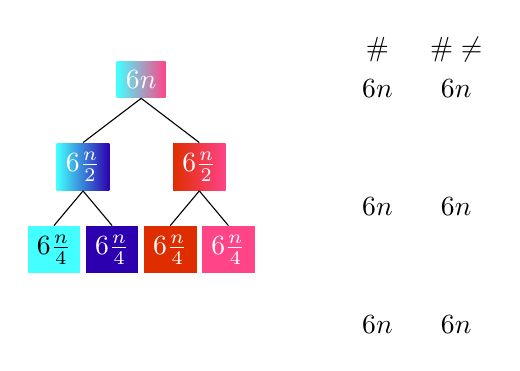
\begin{tikzpicture}
\Tree
[ .\node[shading = axis, left color=nodeblue1, right color=nodered2,shading angle=90, text=white]{$6n$};    
[.\node[shading = axis, left color=nodeblue1, right color=nodeblue2,shading angle=90, text=white]{$6\frac{n}{2}$};
 [.\node(n3l)[fill=nodeblue1]{$6\frac{n}{4}$};]
 [.\node[fill=nodeblue2, text=white]{$6\frac{n}{4}$};]
]
[.\node[shading = axis, left color=nodered1, right color=nodered2,shading angle=90, text=white]{$6\frac{n}{2}$};
 [.\node[fill=nodered1, text=white]{$6\frac{n}{4}$};]
 [.\node(n3r)[fill=nodered2, text=white]{$6\frac{n}{4}$};]
]
]
\node at (3,0.5) {$\#$};
\node at (4,0.5) {$\# \neq$};
\node at (3,0) {$6n$};
\node at (3,-1.5) {$6n$};
\node at (3,-3) {$6n$};
\node at (4,0) {$6n$};
\node at (4,-1.5) {$6n$};
\node at (4,-3) {$6n$};
\end{tikzpicture}
}
\caption{$\symKd$ boom}
\label{fig:splitsingsvlakken-kd}
\end{subfigure}
\begin{subfigure}[t]{.3\linewidth}
\resizebox{\textwidth}{!}{%
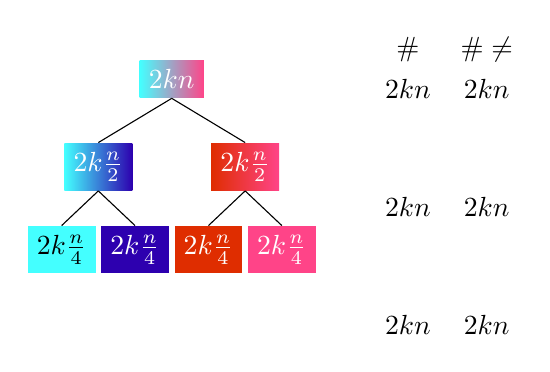
\begin{tikzpicture}
\Tree
[ .\node[shading = axis, left color=nodeblue1, right color=nodered2,shading angle=90, text=white]{$2kn$};    
[.\node[shading = axis, left color=nodeblue1, right color=nodeblue2,shading angle=90, text=white]{$2k\frac{n}{2}$};
 [.\node(n3l)[fill=nodeblue1]{$2k\frac{n}{4}$};]
 [.\node[fill=nodeblue2, text=white]{$2k\frac{n}{4}$};]
]
[.\node[shading = axis, left color=nodered1, right color=nodered2,shading angle=90, text=white]{$2k\frac{n}{2}$};
 [.\node[fill=nodered1, text=white]{$2k\frac{n}{4}$};]
 [.\node(n3r)[fill=nodered2, text=white]{$2k\frac{n}{4}$};]
]
]
\node at (3,0.5) {$\#$};
\node at (4,0.5) {$\# \neq$};
\node at (3,0) {$2kn$};
\node at (3,-1.5) {$2kn$};
\node at (3,-3) {$2kn$};
\node at (4,0) {$2kn$};
\node at (4,-1.5) {$2kn$};
\node at (4,-3) {$2kn$};
\end{tikzpicture}
}
\caption{$\symRBSP$ boom}
\label{fig:splitsingsvlakken-rbsp}
\end{subfigure}
\begin{subfigure}[t]{.3\linewidth}
\resizebox{\textwidth}{!}{%
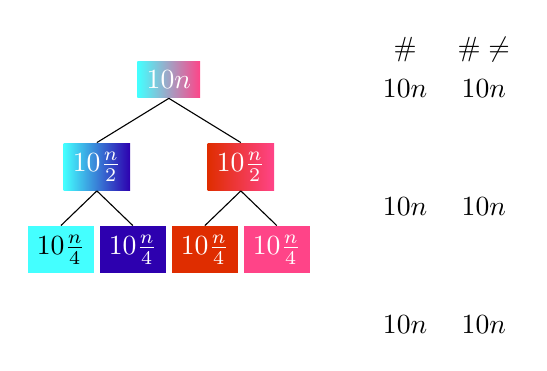
\begin{tikzpicture}
\Tree
[ .\node[shading = axis, left color=nodeblue1, right color=nodered2,shading angle=90, text=white]{$10n$};    
[.\node[shading = axis, left color=nodeblue1, right color=nodeblue2,shading angle=90, text=white]{$10\frac{n}{2}$};
 [.\node(n3l)[fill=nodeblue1]{$10\frac{n}{4}$};]
 [.\node[fill=nodeblue2, text=white]{$10\frac{n}{4}$};]
]
[.\node[shading = axis, left color=nodered1, right color=nodered2,shading angle=90, text=white]{$10\frac{n}{2}$};
 [.\node[fill=nodered1, text=white]{$10\frac{n}{4}$};]
 [.\node(n3r)[fill=nodered2, text=white]{$10\frac{n}{4}$};]
]
]
\node at (3,0.5) {$\#$};
\node at (4,0.5) {$\# \neq$};
\node at (3,0) {$10n$};
\node at (3,-1.5) {$10n$};
\node at (3,-3) {$10n$};
\node at (4,0) {$10n$};
\node at (4,-1.5) {$10n$};
\node at (4,-3) {$10n$};
\end{tikzpicture}
}
\caption{$\symBSPize$ boom}
\label{fig:splitsingsvlakken-bspize}
\end{subfigure}
\caption{Per niveau het aantal ($\#$) splitsingsvlakken en het totaal aantal verschillende ($\# \neq$) splitsingsvlakken gebruikt in bovenliggende niveaus.}
%TODO: meer uitleg
\end{figure}

%%% Local Variables: 
%%% mode: latex
%%% TeX-master: "masterproef"
%%% End: 

\chapter{$\symBSPsweep$}
\label{hoofdstuk:bsp-sweep}
In dit hoofdstuk wordt een nieuwe soort $\symBSP$ boom besproken: de $\symBSPsweep$ boom.
Eerst wordt het algemene idee besproken en nadien een aantal specifieke versies van de $\symBSPsweep$.

% Duidelijk wiskundig uitleggen

 % TODO
 % Beginnen met het probleem te schetsen, aantal paragrafen aan spenderen: 
%  	- Eerst uitleggen in welke gevallen het nuttig is dat je die vrijheid gebruikt
%	- In dit soort scene, intuitief ...

\section{Probleemstelling}
    Het doel van acceleratiestructuren is om de totale kost om een scene te renderen, te minimaliseren.
    Deze rendertijd $\symTime_{\symRender}$ bestaat uit twee grote factoren: de tijd gespendeerd aan het intersecteren met driehoeken (de intersectietijd) en de tijd gespendeerd aan het doorkruisen van de boom (de doorkruistijd).
    De totale intersectietijd $\symTime_{\symIntersection, \symTotal}$ is afhankelijk van het aantal driehoeken $\symNbPrimitives_\symLeaf$ in de geïntersecteerde bladknopen $\symLeaf$ en het aantal keer $\symTraversalL_\symLeaf$ dat elk van deze bladknopen doorkruist wordt.
    De totale doorkruistijd $\symTime_{\symTraversal, \symTotal}$ is afhankelijk van het aantal doorkruisingen $\symTraversalL_{\symInternal}$ van inwendige knopen.
    Formule \ref{eq:rendertijd} beschrijft dit wiskundig met $\symTime_{\symIntersection}$ de tijd nodig voor één straal-driehoek intersectie en $\symTime_{\symTraversal}$ de tijd nodig om één knoop te doorkruisen. 
\begin{equation}
    \label{eq:rendertijd}
   \symTime_{\symRender} \sim
    \symTime_{\symIntersection, \symTotal} + \symTime_{\symTraversal, \symTotal} = \symTime_{\symIntersection} * \sum_{\symLeaf}^\symLeafL \symNbPrimitives_\symLeaf * \symTraversalL_\symLeaf + \symTime_{\symTraversal} * \symTraversalL_{\symInternal}
\end{equation}

Stel dat één kindknoop $\symLeaf_j$ uit de boom wordt opgesplitst in twee kleinere kindknopen $\symLeaf_{j1}$ en $\symLeaf_{j2}$ die elk de helft van de driehoeken krijgen.
Deze opsplitsing is voordelig als aan voorwaarde \ref{eq:vw_splitwinst} voldaan is.
Deze voorwaarde drukt uit dat knoop $\symLeaf_j$ nu een inwendig knoop wordt en dus niet meer zorgt voor een intersectietijd en wel voor een doorkruistijd en dat de nieuwe kindknopen zorgen voor een intersectietijd.
De voorwaarde is equivalent aan voorwaarden \ref{eq:vw_splitwinst_tussen} en \ref{eq:vw_splitwinst_res}.
% B -> 2Bs : nb -> nb/2 * 2 en Db1 + db2 << Db + 1 inwendige knoop, Db keer bekeken
\begin{equation}
    \label{eq:vw_splitwinst}
    \symTime_{\symRender} - \symTime_{\symIntersection} * \symNbPrimitives_{\symLeaf_j} * \symTraversalL_{\symLeaf_j} + \symTime_{\symTraversal} * \symTraversalL_{\symLeaf_j}  + \frac{\symNbPrimitives_{\symLeaf_j}}{2} * (\symTraversalL_{\symLeaf_{j1}} + \symTraversalL_{\symLeaf_{j2}}) * \symTime_{\symIntersection} \leq \symTime_{\symRender}
\end{equation}
\begin{equation}
    \label{eq:vw_splitwinst_tussen}
  \Leftrightarrow \frac{\symNbPrimitives_{\symLeaf_j}}{2} * (\symTraversalL_{\symLeaf_{j1}} + \symTraversalL_{\symLeaf_{j2}}) * \symTime_{\symIntersection} \leq (\symTime_{\symIntersection} * \symNbPrimitives_{\symLeaf_j} - \symTime_{\symTraversal}) * \symTraversalL_{\symLeaf_j}
\end{equation}
%\begin{equation}
%    \frac{\symNbPrimitives_{\symLeaf_j} * \symTime_{\symIntersection}}{(\symTime_{\symIntersection} * \symNbPrimitives_{\symLeaf_j} - \symTime_{\symTraversal})} \leq \frac{2\symTraversalL_{\symLeaf_j}}{(\symTraversalL_{\symLeaf_{j1}} + \symTraversalL_{\symLeaf_{j2}}) }
%\end{equation}
%\begin{equation}
%    \frac{1}{(1 - \frac{\symTime_{\symTraversal}}{\symNbPrimitives_{\symLeaf_j} * \symTime_{\symIntersection}})} \leq \frac{2\symTraversalL_{\symLeaf_j}}{(\symTraversalL_{\symLeaf_{j1}} + \symTraversalL_{\symLeaf_{j2}}) }
%\end{equation}
\begin{equation}
    \label{eq:vw_splitwinst_res}
    \Leftrightarrow \symTraversalL_{\symLeaf_{j1}} + \symTraversalL_{\symLeaf_{j2}} \leq
    2\symTraversalL_{\symLeaf_j} * (1 - \frac{\symTime_{\symTraversal}}{\symNbPrimitives_{\symLeaf_j} * \symTime_{\symIntersection}})
\end{equation}

De som in het linkerlid van voorwaarde \ref{eq:vw_splitwinst_res} is minstens gelijk aan $\symTraversalL_{\symLeaf_{j}}$ aangezien elke doorkruising van $\symLeaf_j$ voor minstens één doorkruising door een kindknoop zorgt.
Analoog kan worden ingezien dat de maximale waarde voor deze som gelijk is aan $2\symTraversalL_{\symLeaf_{j}}$ aangezien elke doorkruising van $\symLeaf_j$ voor maximaal twee doorkruisingen door een kindknoop kan zorgen. Hieruit volgt ongelijkheid \ref{eq:vw_doorkruisingen}.

\begin{equation}
    \label{eq:vw_doorkruisingen}
    \symTraversalL_{\symLeaf_{j}} \leq \symTraversalL_{\symLeaf_{j1}} + \symTraversalL_{\symLeaf_{j2}} \leq 2\symTraversalL_{\symLeaf_{j}}
\end{equation}

In het algemeen geval geldt dat $\symTraversalL_{\symLeaf_{j1}} + \symTraversalL_{\symLeaf_{j2}} = (2 * (1-\alpha) + \alpha) \symTraversalL_{\symLeaf_{j}}$ waarbij $\alpha$ het procentueel aantal doorkruisingen is dat door slechts één van de twee kindknopen gaat.
In dit geval leidt voorwaarde \ref{eq:vw_splitwinst_res} tot voorwaarde \ref{eq:vw_splitwinst_general}.
\begin{equation}
    \label{eq:vw_splitwinst_general}
    (2 * (1-\alpha) + \alpha) \symTraversalL_{\symLeaf_{j}} \leq
    2\symTraversalL_{\symLeaf_j} - \frac{2\symTraversalL_{\symLeaf_j}\symTime_{\symTraversal}}{\symNbPrimitives_{\symLeaf_j} \symTime_{\symIntersection}}
    \Leftrightarrow
    2 - \alpha \leq 2 - \frac{2\symTime_{\symTraversal}}{\symNbPrimitives_{\symLeaf_j} \symTime_{\symIntersection}}
    \Leftrightarrow
    \symTime_{\symTraversal} \leq \frac{\alpha \symNbPrimitives_{\symLeaf_j} }{2}\symTime_{\symIntersection}
\end{equation}

In het ideale geval ($\alpha = 1$) leidt voorwaarde \ref{eq:vw_splitwinst_general} tot $\symTime_{\symTraversal} \leq \frac{\symNbPrimitives_{\symLeaf_j}}{2}\symTime_{\symIntersection}$.
Het opsplitsen van een knoop met twee elementen, kan hierdoor pas voordelig zijn als de doorkruistijd kleiner is dan de intersectietijd.
Aangezien de doorkruistijd in de realiteit beduidend kleiner is dan de intersectietijd, is het in dit ideale geval altijd voordelig om een kindknoop op te splitsen, ongeacht het aantal driehoeken in de knoop.
In het slechtste geval ($\alpha = 0$) kan aan voorwaarde \ref{eq:vw_splitwinst_general} enkel voldaan zijn als de doorkruistijd gelijk is aan nul. Dit is onmogelijk waardoor opsplitsen nooit voordelig kan zijn in dit geval. \\

Het is moeilijk om de waarde van $\alpha$ te voorspellen, deze is namelijk afhankelijk van de exacte stralen die tijdens het renderen gevolgd worden, de specifieke driehoeken in de knoop en het splitsingsvlak. Voorwaarde \ref{eq:vw_splitwinst_general} toont dat de kans dat splitsen voordelig is, lineair stijgt met $\symNbPrimitives_{\symLeaf_j}$. De voorwaarde toont ook dat het splitsen van een knoop met twee driehoeken, voordelig is wanneer de doorkruistijd $\alpha$ keer kleiner is dan de intersectietijd. Intuitief lijkt het logisch dat hier in het algemeen aan voldaan is. Hieruit kan worden afgeleid dat het altijd beter is om bladknopen met meer dan één driehoek op te splitsen in twee kleinere bladknopen. De volgende secties ... \\



\section{Algemeen idee}
    De $\symBSPsweep$ boom is een algemene $\symBSP$ boom waarbij in elke knoop k richtingen bepaald worden en alle $2n$ splitsingsvlakken langs elk van deze richtingen worden bekeken door te sweepen.
    Deze k richtingen kunnen verschillend zijn voor elke knoop en kunnen gekozen worden afhankelijk van de lokale geometrie.
    De $\symRBSP$ boom is een $\symBSPsweep$ boom waarbij de gekozen richtingen in elke knoop hetzelfde zijn.
    De $\symBSPsweep$ boom heeft drie belangrijke ontwerpbeslissingen.
    De belangrijkste ontwerpbeslissing bij de $\symBSPsweep$ boom is de methode die gebruikt wordt om de k richtingen te bepalen.
    Een tweede belangrijke ontwerpbeslissing is de waarde van k.
    De derde belangrijke ontwerpbeslissing sluit aan bij de eerst en gaat over het al dan niet gebruiken van de $\symKd$ richtingen als de eerste drie van de k richtingen.
    \\


    %Kd-richtingen + aantal richtingen of puur die richtingen
    %Snelle traversal voor kd-richtingen
\section{Gebaseerd op random richtingen}
De simpelste $\symBSPsweep$ bepaalt in elke knoop k random richtingen onafhankelijk van de geometrie.
De richtingen worden uniform op de hemisphere gegenereerd.
Het idee achter deze boom is dat het nuttiger kan zijn om driehoeken via veel verschillende vlakken te proberen splitsen, dan om ze steeds met dezelfde vlakken te proberen splitsen.
Als de driehoeken in de scene uniform verdeeld zijn, dan is de kans dat twee driehoeken volgens een willekeurige richting gesplitst kunnen worden, even groot als de kans dat ze door een $\symKd$ richting gesplitst kunnen worden.

Als de $\symBSPrandom$ boom perfect gebalanceerd is, worden in elk niveau $2kn$ verschillende splitsingsvlakken bekeken.
Deze splitsingsvlakken zijn verschillend op elk niveau, zodat in totaal $2knlog(n)$ verschillende splitsingsvlakken bekeken worden.
Figuur \ref{fig:splitsingsvlakken-bsprandom} toont dit visueel.
De $\symBSPrandom$ boom probeert elke driehoek via gemiddeld $2klog(n)$ ($\symO(log(n))$) vlakken te splitsen van de andere driehoeken, in tegenstelling tot de bestaande bomen die dit maximaal met $\symO(1)$ vlakken proberen.\\

\begin{figure}
    \centering

   \resizebox{0.4\textwidth}{!}{%
   \centering
    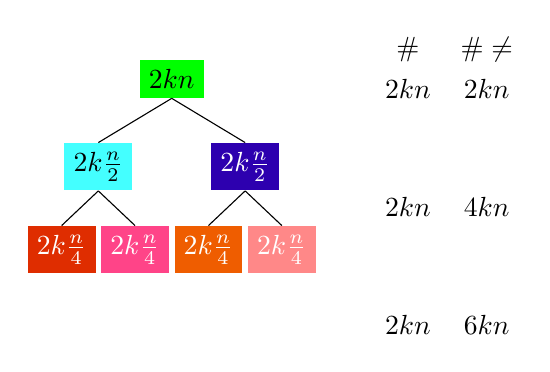
\begin{tikzpicture}
   \Tree
   [ .\node[fill=green]{$2kn$};    
       [.\node[fill=nodeblue1]{$2k\frac{n}{2}$};
           [.\node(n3l)[fill=nodered1, text=white]{$2k\frac{n}{4}$};]
           [.\node[fill=nodered2, text=white]{$2k\frac{n}{4}$};]
       ]
       [.\node[fill=nodeblue2, text=white]{$2k\frac{n}{2}$};
           [.\node[fill=nodered3, text=white]{$2k\frac{n}{4}$};]
           [.\node(n3r)[fill=nodered4, text=white]{$2k\frac{n}{4}$};]
       ]
   ]
   \node at (3,0.5) {$\#$};
   \node at (4,0.5) {$\# \neq$};
   \node at (3,0) {$2kn$};
   \node at (3,-1.5) {$2kn$};
   \node at (3,-3) {$2kn$};
   \node at (4,0) {$2kn$};
   \node at (4,-1.5) {$4kn$};
   \node at (4,-3) {$6kn$};
   \end{tikzpicture}
   }
   \caption[Splitsingsvlakken $\symBSPrandom$]%
    {Splitsingsvlakken $\symBSPrandom$ - \small Per niveau het aantal ($\#$) splitsingsvlakken en het totaal aantal verschillende ($\# \neq$) splitsingsvlakken gebruikt in bovenliggende niveaus bij de $\symBSPrandom$ boom.} %TODO: meer uitleg
    \label{fig:splitsingsvlakken-bsprandom}
\end{figure}

\begin{figure}
        \resizebox{\textwidth}{!}{%
        \centering
         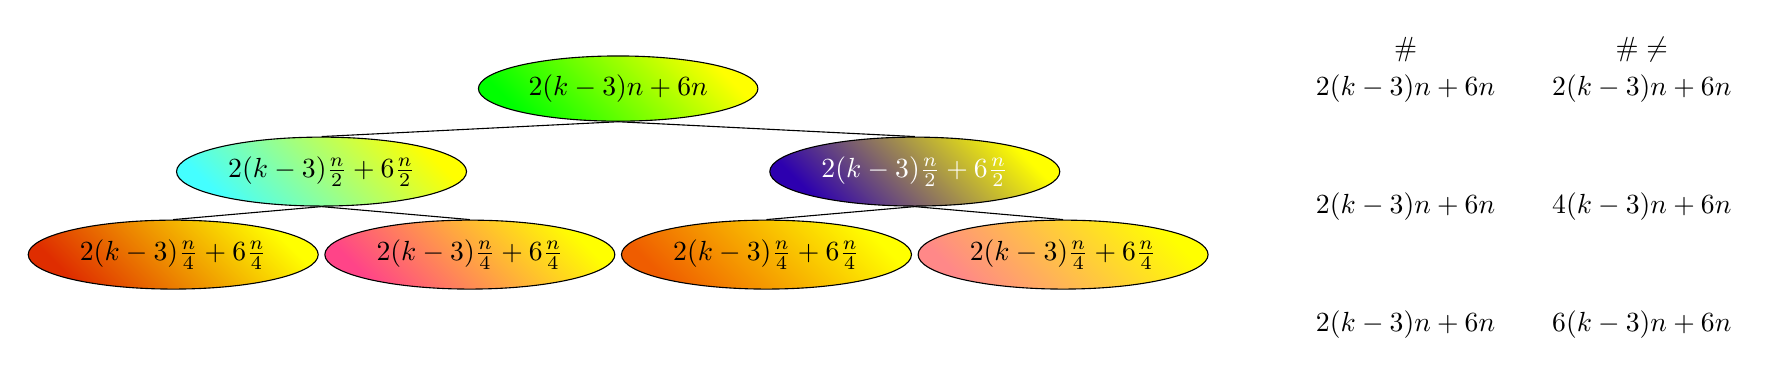
\begin{tikzpicture}
            \usetikzlibrary{arrows}
            \usetikzlibrary{shapes}
\tikzstyle{every tree node}=[draw, ellipse, align=center]
        \Tree
        [ .\node[shading = axis, left color=green, right color=nodeyellow1,shading angle=135]{$2(k-3)n + 6n$};    
            [.\node[shading = axis, left color=nodeblue1, right color=nodeyellow1, shading angle=135]{$2(k-3)\frac{n}{2} + 6\frac{n}{2}$};
                [.\node(n3l)[shading = axis, left color=nodered1, right color=nodeyellow1, shading angle=135]{$2(k-3)\frac{n}{4} + 6\frac{n}{4}$};]
                [.\node[shading = axis, left color=nodered2, right color=nodeyellow1, shading angle=135]{$2(k-3)\frac{n}{4} + 6\frac{n}{4}$};]
            ]
            [.\node[shading = axis, left color=nodeblue2, right color=nodeyellow1, shading angle=135, text=white]{$2(k-3)\frac{n}{2} + 6\frac{n}{2}$};
                [.\node[shading = axis, left color=nodered3, right color=nodeyellow1, shading angle=135]{$2(k-3)\frac{n}{4} + 6\frac{n}{4}$};]
                [.\node(n3r)[shading = axis, left color=nodered4, right color=nodeyellow1, shading angle=135]{$2(k-3)\frac{n}{4} + 6\frac{n}{4}$};]
            ]
        ]
        \node at (10,0.5) {$\#$};
        \node at (13,0.5) {$\# \neq$};
        \node at (10,0) {$2(k-3)n + 6n$};
        \node at (10,-1.5) {$2(k-3)n + 6n$};
        \node at (10,-3) {$2(k-3)n + 6n$};
        \node at (13,0) {$2(k-3)n + 6n$};
        \node at (13,-1.5) {$4(k-3)n + 6n$};
        \node at (13,-3) {$6(k-3)n + 6n$};
        \end{tikzpicture}
        }
    \caption[Splitsingsvlakken $\symBSPrandomsomekd$]%
    {Splitsingsvlakken $\symBSPrandomsomekd$ - \small Per niveau het aantal ($\#$) splitsingsvlakken en het totaal aantal verschillende ($\# \neq$) splitsingsvlakken gebruikt in bovenliggende niveaus bij de $\symBSPrandomsomekd$ boom.} %TODO: meer uitleg
    \label{fig:splitsingsvlakken-bsprandomsomekd}
\end{figure}

De $\symKd$ richtingen zijn in praktische scenes vaak beter dan willekeurige richtingen omdat ze loodrecht op elkaar staan waardoor ze de hemisphere goed bedekken.
Dit geeft aanleiding tot een boom die als eerste drie richtingen steeds de $\symKd$ richtingen kiest en enkel de overige $k - 3$ richtingen random genereert: de $\symBSPrandomkd$ boom. Een extra voordeel is dat de snellere $\symKd$ knoop doorkruising gebruikt kan worden. Een boom die altijd de $\symKd$ richtingen gebruikt en de doorkruising van $\symKd$ knopen optimaliseert, wordt aangeduid als $\symBSPrandomfastkd$. 
Als de $\symBSPrandomsomekd$ boom perfect gebalanceerd is, worden in elk niveau $2kn$ splitsingsvlakken bekeken.
Van deze $2kn$ zijn er $6n$ die hergebruikt worden, de vlakken volgens de $\symKd$ richtingen.
Dit zorgt voor $2(k-3)n$ verschillende splitsingsvlakken per niveau, zodat in totaal $2(k-3)nlog(n) + 6n$ verschillende splitsingsvlakken bekeken worden.
Figuur \ref{fig:splitsingsvlakken-bsprandomsomekd} toont dit visueel.
De $\symBSPrandomsomekd$ boom probeert elke driehoek via gemiddeld $\symO(log(n))$ vlakken te splitsen van de andere driehoeken, net als  de $\symBSPrandom$ boom.\\


%(Extra) richtingen door random richtingen te kiezen
%Ter controle dat de richtingen met behulp van normalen, nuttige richtingen zijn
%Sweeping
%Waarom zou dit werken ? : Random per node itt vast bij Kd
%    Driehoeken proberen te worden gesplitst volgens meer verschillende richtingen, Kd probeert steeds hetzelfde
%    Kd heeft maar 3 opties, als het volgens geen kan -> nooit mogelijk
%    Kans splitsbaar door Kd richting of random is even hoog in uniform geval. Scenes hebben wel veel asgealigneerde delen, dus daarom die extra.

\section{Gebaseerd op geometrische normalen}
\subsection{Willekeurige normaal}
    Extra richtingen door random normalen te kiezen
    Autopartitie van Ize maar gesweeped
    Waarom zou dit werken ? : ...
    
\subsection{Geclusterde normalen}
    (Extra) richtingen via K-means clustering
    Sweepen volgens die richtingen
    Waarom zou dit werken ...

%\section{Hiërarchie}


%%% Local Variables: 
%%% mode: latex
%%% TeX-master: "masterproef"
%%% End: 
\chapter{Implementatie}
\label{hoofdstuk:implementatie}
In dit hoofdstuk wordt de implementatie van volgende $\symBSP$ bomen besproken: $\symKd$ boom, $\symRBSP$ boom, $\symRBSPKd$ boom, $\symBSPize$ boom, $\symBSPizefastkd$ boom, $\symBSPrandom$ boom, $\symBSPrandomkd$ boom, $\symBSPrandomfastkd$ boom, $\symBSParbitrary$ boom, $\symBSParbitrarykd$ boom, $\symBSParbitraryfastkd$ boom, $\symBSPcluster$ boom, $\symBSPclusterkd$ boom en $\symBSPclusterfastkd$ boom. \\

Het hoofdstuk start met een hoogniveau beschrijving (\ref{sec:h4-hoog-niveau}) van het algoritme om de boom te bouwen en het algoritme om de boom te intersecteren.
Daarna wordt voor elk type boom besproken hoe hun knopen worden voorgesteld in het geheugen (\ref{sec:h4-voorstelling-knopen}.
De specifieke implementaties van de bouwalgoritmes (\ref{sec:h4-bouwalgoritmes}) en intersectie-algoritmes (\ref{sec:h4-intersectie-algoritmes}) worden dan besproken.



%\section{Outline BSP-algoritmes}
%\section{Datastructuren knopen}
%\section{Bouwalgoritmes}
%    \subsection{SAH}
    %Intersectie willekeurig vlak & asgealigneerd
    % Snellere intersect / aangepast SAH
%\section{Intersectie-algoritmes}
\definecolor{codegreen}{rgb}{0,0.6,0}
\definecolor{codegray}{rgb}{0.5,0.5,0.5}
\definecolor{codepurple}{rgb}{0.58,0,0.82}
\definecolor{backcolor}{rgb}{0.95,0.95,0.92}
\lstdefinestyle{pseudoStyle}{
    backgroundcolor=\color{backcolor},   
    numberstyle=\tiny\color{codegray},
    stringstyle=\color{codepurple},
    %basicstyle=\footnotesize,
    breakatwhitespace=false,         
    breaklines=true,                 
    captionpos=b,                    
    keepspaces=true,                 
    numbers=left,                    
    numbersep=5pt,                  
    showspaces=false,                
    showstringspaces=false,
    showtabs=false,                  
    tabsize=2,
    basicstyle=\fontsize{9}{11}\selectfont\ttfamily
}
\lstset{style=pseudoStyle}

%TODO: slechteAanpassingen
\section{Hoog niveau beschrijving}
\label{sec:h4-hoog-niveau}
\subsection{Bouwalgoritme}
Het bouwalgoritme voor $\symBSP$ bomen heeft een aantal parameters:
\begin{itemize}
    \item $\symCost_\symIntersection$: De intersectiekost voor primitieven. Deze parameter is nodig voor de $\symSAH$ heuristiek.
    \item $\symCostTraversalKd$: De doorkruiskost voor $\symKd$ knopen. Deze parameter is nodig voor de $\symSAH$ heuristiek.
    \item $\symCostTraversalBSP$: De aparte doorkruiskost voor $\symBSP$ knopen. Deze parameter is nodig voor de $\symSAH$ heuristiek.
    \item $\symMaxPrims$: Elke knoop met $\symMaxPrims$ of minder primitieven wordt direct een bladknoop, er wordt niet geprobeerd om de knoop te splitsen.
    \item $\symMaxDepth$: De maximale diepte van de boom.
\end{itemize}
\begin{dutchalgorithm}
    \begin{algorithmic}

        \State $stack\gets \emptyset$
        \State Voeg een bouwknoop met alle primitieven toe aan de stack
        \While {$stack \neq \emptyset$}
            \State $b \gets $\Call{pop}{$stack$}
            \If {$b_{\symNbPrimitives} \leq \symMaxPrims$ \Or $b_{d} = \symMaxDepth$}
                \State \Call{maak\_blad\_knoop}{b}
                \State $continue$
            \EndIf
            \State $besteSplit \gets $ \Call{bepaal\_beste\_split}{b}
            \State $nietSplitKost \gets  b_{\symNbPrimitives}*\symCost_\symIntersection$
            \If {$besteSplit_{kost} > nietSplitKost$}
                \State $b_{slechteAanpassingen} \gets b_{slechteAanpassingen} + 1$
            \EndIf
            \If {$(besteSplit_{kost} > 4 * nietSplitKost$ \And $b_{\symNbPrimitives} < 16)$ \Or $besteSplit = None$ \Or $b_{slechteAanpassingen} = 3$}
                \State \Call{maak\_blad\_knoop}{b}
                \State $continue$
            \EndIf
            \State \Call{maak\_inwendige\_knoop}{b}
            \State Plaats de kindknopen als twee nieuwe bouwknopen op de stack
        \EndWhile
    \end{algorithmic}
    \caption{Bouwen van een BSP boom}
\end{dutchalgorithm}

\subsection{Intersectie-algoritme}
Een straal wordt geparameteriseerd als $o + td$.

\begin{dutchalgorithm}
    \begin{algorithmic}       
        \Function{intersecteer}{Boom b, Straal s}
            \State $geraakt_{omhullendVolume}, tMin, tMax \gets $ \Call{intersecteer}{$b_{omhullendVolume}$, s}
            \If {not $geraakt_{omhullendVolume}$}
                \State \Return false
            \EndIf
            \State $geraakt \gets false$
            \State $k \gets b_{wortelKnoop}$
            \State $stack\gets \emptyset$

            \While {$k \neq None$}
                \If {$s_{maxT} < tMin$}
                    \State $break$
                \EndIf
                \If {\Call{is\_inwendige\_knoop}{k}}
                    \State $tVlak, linksEerst \gets$ \Call{intersecteer\_inwendige\_knoop}{k,s}
                    \If {$linksEerst$}
                        \State $k_1 \gets k_{linkerKind}$
                        \State $k_2 \gets k_{rechterKind}$
                    \Else
                        \State $k_1 \gets k_{rechterKind}$
                        \State $k_2 \gets k_{linkerKind}$
                    \EndIf
                    \If {$tVlak > tMax$ \Or $tVlak <= 0$}
                        \State $k \gets k_1$
                    \ElsIf {$tVlak < tMin$}
                        \State $k \gets k_2$
                    \Else
                        \State \Call{add}{$stack, \{k_2, tMin: tVlak, tMax: tMax\})$}
                        \State $k \gets k_1$
                        \State $tMax \gets tVlak$ 
                    \EndIf
                \Else
                    \If {\Call{intersecteer\_bladknoop}{k, s}}
                        \State $geraakt \gets true$
                    \EndIf
                    \If {$stack \neq \emptyset$}
                        \State $k, tMin, tMax \gets $\Call{pop}{$stack$}
                    \Else
                        \State $break$
                    \EndIf
                \EndIf
            \EndWhile
            \State \Return $geraakt$
        \EndFunction
    \end{algorithmic}
    \caption{Intersecteren van een BSP boom}
\end{dutchalgorithm}
    
\begin{dutchalgorithm}
    \begin{algorithmic}       
        \Function{intersecteer\_inwendige\_knoop}{$\symKd$ Knoop k, Straal s}
            \State $as <- k_{splitsAs}$
            \State $tVlak \gets $ \Call{kd\_vlak\_afstand}{$k_{splitPos}$, s, $\frac{1}{\vec{s_d}}$, as}
            \State $linksEerst \gets \vec{s_o}[as] < k_{splitPos}$ \Or $(\vec{s_o}[as] = k_{splitPos}$ \And $s_d[as] \leq 0)$
            \State \Return $tVlak$, $linksEerst$
        \EndFunction
    \end{algorithmic}
    \caption{Intersecteren van een inwendige $\symKd$ knoop.}
\end{dutchalgorithm}

\begin{dutchalgorithm}
    \begin{algorithmic}       
        \Function{kd\_vlak\_afstand}{splitPositie, s, inverseRichting, as}
            \State \Return $(splitPos - \vec{s_o}[as]) * \vec{inverseRichting}[as]$
        \EndFunction
    \end{algorithmic}
    \caption{Intersectie tussen een asgealigneerd vlak en een straal.}
\end{dutchalgorithm}

\begin{dutchalgorithm}
    \begin{algorithmic}       
        \Function{intersecteer\_inwendige\_knoop}{$\symRBSP$ Knoop k, Straal s}
            \State $richtingId \gets k_{splitsAs}$
            \State $tVlak, projOorsprong, invProjRichting \gets $ \Call{vlak\_afstand}{$\vec{richtingen[richtingId]}$, $k_{splitPos}$, s}
            \State $linksEerst \gets projOorsprong < k_{splitPos}$ \Or $(projOorsprong = k_{splitPos}$ \And $invProjRichting \leq 0)$
            \State \Return $tVlak$, $linksEerst$
        \EndFunction
    \end{algorithmic}
    \caption{Intersecteren van een inwendige $\symRBSP$ knoop.}
\end{dutchalgorithm}

\begin{dutchalgorithm}
    \begin{algorithmic}       
        \Function{intersecteer\_inwendige\_knoop}{$\symRBSPKd$ Knoop k, Straal s}
            \State $richtingId \gets k_{splitsAs}$
            \If {$richtingId < 3$}
                \State $tVlak \gets $ \Call{kd\_vlak\_afstand}{$k_{splitPos}$, s, $\frac{1}{\vec{s_d}}$, richtingId}
                \State $linksEerst \gets \vec{s_o}[richtingId] < k_{splitPos}$ \Or $(\vec{s_o}[richtingId] = k_{splitPos}$ \And $s_d[richtingId] \leq 0)$
                \State \Return $tVlak$, $linksEerst$
            \Else
                \State $tVlak, projOorsprong, invProjRichting \gets $ \Call{vlak\_afstand}{$\vec{richtingen[richtingId]}$, $k_{splitPos}$, s}
                 \State $linksEerst \gets projOorsprong < k_{splitPos}$ \Or $(projOorsprong = k_{splitPos}$ \And $invProjRichting \leq 0)$
                \State \Return $tVlak$, $linksEerst$
            \EndIf
        \EndFunction
    \end{algorithmic}
    \caption{Intersecteren van een inwendige $\symRBSPKd$ knoop.}
\end{dutchalgorithm}

\begin{dutchalgorithm}
    \begin{algorithmic}       
        \Function{intersecteer\_inwendige\_knoop}{$\symBSP$ Knoop k, Straal s}
            \State $tVlak, projOorsprong, invProjRichting \gets $ \Call{vlak\_afstand}{$\vec{k_{splitsRichting}}$, $k_{splitPos}$, s}
            \State $linksEerst \gets projOorsprong < k_{splitPos}$ \Or $(projOorsprong = k_{splitPos}$ \And $invProjRichting \leq 0)$
            \State \Return $tVlak$, $linksEerst$
        \EndFunction
    \end{algorithmic}
    \caption{Intersecteren van een inwendige $\symBSP$ knoop.}
\end{dutchalgorithm}

\begin{dutchalgorithm}
    \begin{algorithmic}       
        \Function{intersecteer\_inwendige\_knoop}{$\symBSPKd$ Knoop k, Straal s}
            \State $isKdKnoop \gets k_{flags} < 4$
            \If {$isKdKnoop$}
                \State $as \gets k_{flags}$
                \State $tVlak \gets $ \Call{kd\_vlak\_afstand}{$k_{splitPos}$, s, $\frac{1}{\vec{s_d}}$, as}
                \State $linksEerst \gets \vec{s_o}[as] < k_{splitPos}$ \Or $(\vec{s_o}[as] = k_{splitPos}$ \And $s_d[as] \leq 0)$
                \State \Return $tVlak$, $linksEerst$
            \Else
                \State $tVlak, projOorsprong, invProjRichting \gets $ \Call{vlak\_afstand}{$\vec{k_{splitsRichting}}$, $k_{splitPos}$, s}
                 \State $linksEerst \gets projOorsprong < k_{splitPos}$ \Or $(projOorsprong = k_{splitPos}$ \And $invProjRichting \leq 0)$
                \State \Return $tVlak$, $linksEerst$
            \EndIf
        \EndFunction
    \end{algorithmic}
    \caption{Intersecteren van een inwendige $\symBSPKd$ knoop.}
\end{dutchalgorithm}

\begin{dutchalgorithm}
    \begin{algorithmic}       
        \Function{vlak\_afstand}{$\vec{normaal}$, splitPositie, s}
            \State $projOorsprong \gets \vec{normaal} \cdot \vec{s_o}$
            \State $invProjRichting \gets \frac{1}{\vec{normaal} \cdot \vec{s_d}}$
            \State $afstand \gets (splitPos - projOorsprong) * invProjRichting $
            \State \Return projOorsprong, invProjRichting, afstand
        \EndFunction
    \end{algorithmic}
    \caption{Intersectie tussen een vlak en een straal.}
\end{dutchalgorithm}


\section{Voorstelling knopen}
\label{sec:h4-voorstelling-knopen}
    \begin{table}[tb]
        \begin{subtable}{1\textwidth}
        \centering
        \begin{tabular}{@{}|c|c|c|c|@{}} \toprule      
        Inwendig & bits & Blad & bits \\ \midrule
        tSplit & 32 & primitief Offset & 32 \\
        flags  & 2  &  flags   & 2    \\
        tweedeKindIndex & 30 & $\symNbPrimitives$ & 30 \\ \hline \hline
        & 64 & & 64    \\ \bottomrule
        \end{tabular}
        \caption{$\symKd$ knoop}
        \label{tab:voorstelling-kd-knoop}
        \end{subtable}

        \bigskip
        \begin{subtable}{1\textwidth}
            \centering
            \begin{tabular}{@{}|c|c|c|c|@{}} \toprule      
            Inwendig & bits & Blad & bits \\ \midrule
            tSplit & 32 & primitief Offset & 32 \\
            flags  & $log_2(k + 1)$  &  flags   & $log_2(k + 1)$   \\
            tweedeKindIndex & 32 - $log_2(k + 1)$ & $\symNbPrimitives$ & 32 - $log_2(k + 1)$ \\ \hline \hline
            & 64 & & 64    \\ \bottomrule
            \end{tabular}
            \caption{$\symRBSP$ en $\symRBSPKd$ knoop}
            \label{tab:voorstelling-rbsp-knoop}
        \end{subtable}

        \bigskip
        \begin{subtable}{1\textwidth}
            \centering
            \begin{tabular}{@{}|c|c|c|c|@{}} \toprule      
                Inwendig & bits & Blad & bits \\ \midrule
                tSplit & 32 & primitief Offset & 32 \\
                flags  & 1  &  flags   & 1    \\
                tweedeKindIndex & 31 & $\symNbPrimitives$ & 31 \\
                splitRichting & 96 &  &  \\ \hline \hline
                & 160 & & 64    \\ \bottomrule
            \end{tabular}
            \caption{$\symBSP$ knoop}
            \label{tab:voorstelling-bsp-knoop}
        \end{subtable}

        \bigskip
        \begin{subtable}{1\textwidth}
            \centering
            \begin{tabular}{@{}|c|c|c|c|@{}} \toprule      
                Inwendig & bits & Blad & bits \\ \midrule
                tSplit & 32 & primitief Offset & 32 \\
                flags  & 3  &  flags   & 3   \\
                tweedeKindIndex & 29 & $\symNbPrimitives$ & 29 \\
                splitRichting & 96 &  &  \\ \hline \hline
                & 160 & & 64    \\ \bottomrule
            \end{tabular}
            \caption{$\symBSPKd$ knoop}
            \label{tab:voorstelling-bspkd-knoop}
        \end{subtable}
        \caption[Voorstelling $\symKd$, $\symRBSP$, $\symBSP$ en $\symBSPKd$ knopen]{Voorstelling $\symKd$, $\symRBSP$, $\symBSP$ en $\symBSPKd$ knopen - \small }
    \end{table}                                                                                         

    \begin{table}
        \centering
        \begin{tabular}{@{}|c|c|@{}} \toprule      
        $\symBSP$ boom & Knooptype \\ \midrule
        $\symKd$ & $\symKd$ \\
        $\symRBSP$ & $\symRBSP$  \\
        $\symRBSPKd$ & $\symRBSPKd$  \\
        $\symBSPize$ &  $\symBSP$ \\
        $\symBSPizefastkd$ & $\symBSPKd$ \\
        $\symBSPsweepmaybewithkd$ & $\symBSP$ \\
        $\symBSPsweepkd$ & $\symBSPKd$ \\ \bottomrule
        \end{tabular}
        \caption[Gebruikte soorten knopen voor alle soorten $\symBSP$ bomen]{Gebruikte soorten knopen voor alle soorten $\symBSP$ bomen - \small}
        \label{tab:voorstelling-knoop-boom}
    \end{table}

\section{Bouwalgoritmes}
\label{sec:h4-bouwalgoritmes}


\section{Intersectie-algoritmes}
\label{sec:h4-intersectie-algoritmes}



%
%\section{$\symKd$ boom}
%\section{$\symRBSP$ boom}
%\section{$\symBSPize$}
%\section{$\symBSPsweep$}
%\subsection{Algemeen}
%\subsection{$\symBSPrandom$}
%\subsection{$\symBSParbitrary$}
%\subsection{$\symBSPcluster$}


%%% Local Variables: 
%%% mode: latex
%%% TeX-master: "masterproef"
%%% End: 
\chapter{Resultaten}
\label{hoofdstuk:resultaten}
In dit hoofdstuk wordt het werk ingeleid. Het doel wordt gedefinieerd en er
wordt uitgelegd wat de te volgen weg is (beter bekend als de rode draad).

Als je niet goed weet wat een masterproef is, kan je altijd
Wikipedia eens nakijken.

% Max depth: net zoals Mora en Ka.. gebruiken we k1 * log2(n) + k2 (voorgesteld door Havran en Bittner in [7]) met k1 = 1.2 en k2 = 2
\section{Praktische aspecten}
\section{Afhankelijkheid van aantal richtingen}
\begin{table}
    \centering
    \begin{tabular}{@{}lllllllll@{}} \toprule
      & \multicolumn{2}{c}{Feet} & \multicolumn{2}{c}{Sponza} & \multicolumn{2}{c}{Conference Hall} & \multicolumn{2}{c}{Museum} \\ \cmidrule(r){2-3} \cmidrule(r){4-5} \cmidrule(r){6-7} \cmidrule(r){8-9}
      
      K      & Mediaan     & Stdev & Mediaan & Stdev & Mediaan & Stdev & Mediaan & Stdev \\ \midrule
      4      &     & &     & & & & & \\
      5      &     & &     & & & & & \\
      6      &     & &     & & & & & \\
      7      &     & &     & & & & & \\
      8      &     & &     & & & & & \\
      9      &     & &     & & & & & \\
      10      &     & &     & & & & & \\ \bottomrule
    \end{tabular}
    \caption{Statistieken over de rendertijd voor $\symBSPrandomfastkd$ voor verschillende waarden van K. Voor elke waarde van K is het algoritme 6 keer uitgevoerd. }
    \label{tab:bsprandom-k-rendertijd}
  \end{table}
\section{Vergelijking}


%%% Local Variables: 
%%% mode: latex
%%% TeX-master: "masterproef"
%%% End: 
\chapter{Resultaten}
\label{hoofdstuk:conclusie}


%%% Local Variables: 
%%% mode: latex
%%% TeX-master: "masterproef"
%%% End: 
% Indien er bijlagen zijn:
%\appendixpage*          % indien gewenst
%\appendix
%\include{app-A}
% ... en zo verder tot
%\include{app-n}

\backmatter
% Na de bijlagen plaatst men nog de bibliografie.
% Je kan de  standaard "abbrv" bibliografiestijl vervangen door een andere.
\bibliography{referenties}
\bibliographystyle{alpha}

\end{document}
